
\documentclass{article}
\usepackage{hyperref}
\usepackage[
    type={CC},
    modifier={by-nc-sa},
    version={3.0},
]{doclicense}
\usepackage[landscape]{geometry}
\usepackage{url}
\usepackage{multicol}
\usepackage{mathtools}
\usepackage{amsmath,amssymb}
\usepackage{esint}
\usepackage{amsfonts}
\usepackage{tikz}
\usetikzlibrary{decorations.pathmorphing}
\usepackage{enumitem}
\usepackage{ mathrsfs }
\usepackage{empheq}

\newcommand*\widefbox[1]{\fbox{\hspace{2em}#1\hspace{2em}}}
\newcommand*\bs[1]{\boldsymbol{#1}}


\title{MATH 307}
\usepackage[english]{babel}
\usepackage[utf8]{inputenc}

\advance\topmargin-.8in
\advance\textheight3in
\advance\textwidth3in
\advance\oddsidemargin-1.5in
\advance\evensidemargin-1.5in
\parindent0pt
\parskip2pt
\newcommand{\hr}{\centerline{\rule{3.5in}{1pt}}}
\newcommand\subtopic[1]{
    \textbf{#1}
    \vspace{.1cm}
    \hrule
    \vspace{.2cm}}
    

\begin{document}

\begin{center}{\huge{\textbf{UBC MATH 307}}}\\
\end{center}

\begin{multicols*}{3}

\tikzstyle{mybox} = [draw=black, fill=white, very thick,
    rectangle, rounded corners, inner sep=10pt, inner ysep=10pt]
\tikzstyle{fancytitle} =[fill=black, text=white, font=\bfseries]

 
 %------------ LU Matrix ---------------
\begin{tikzpicture}
\node [mybox] (box){%
    \begin{minipage}{0.3\textwidth}
    \subtopic{Construction}
    Use Gaussian elimination to produce an upper triangular matrix, $U$. The lower triangular matrix $L$ records the inverse of the row reduction operations.  No pivoting of rows allowed.  If $A$ can be reduced by Gaussian elimination to row echelon form only with operations without scaling rows and without interchanging rows, then $A$ has an LU decomposition of the form:
    $$A = LU$$
    
    Where $L$ records the coefficients $c_{i,j}$ for each row reduction operation-- add $c_{i,j}$ times row $j$ to row $i$:
 
$$
L =
\begin{bmatrix}
1 & & & & \\
-c_{2,1} & 1 & & & \\
-c_{3,1} & -c_{3,2} & 1 & & \\
\vdots & \vdots & \ddots & \ddots & \\
-c_{m,1} & -c_{m,2} & \cdots & -c_{m,m-1} & 1
\end{bmatrix}
$$

\subtopic{Back Substitution}
    
    To solve $A \boldsymbol{x} = \boldsymbol{b}$, use the decomposition $LU \boldsymbol{x} = \boldsymbol{b}$
    
    \begin{equation*}
\boxed{
\text{Solve:} L \boldsymbol{y} = \boldsymbol{b}$\text{, then} $U \boldsymbol{x} = \boldsymbol{y} 
}
\end{equation*}

\subtopic{Useful Properties of LU}
    $\begin{aligned}[t]
   \mathrm{rank}(A) & = \mathrm{rank}(U) \\
    \det(A) & = \det(U) = \Pi(\text{Diagonal entries } U)\\
    N(A)&=N(U)\\
    R(A) &= \mathrm{span} \{ \boldsymbol{\ell}_1 , \dots , \boldsymbol{\ell}_r \} \text{for } r = \mathrm{rank}(A),
\end{aligned}$
    \end{minipage}
};
%------------ LU Decomp ---------------------
\node[fancytitle, right=10pt] at (box.north west) {LU Decompositions};
\end{tikzpicture}

%-------------------Authorship-----------------------
\begin{center}
    \framebox{
    \parbox[t][1.5cm]{6.5cm}{
    \addvspace{0.2cm} \centering 
    \footnotesize \textbf{Compiled by Simon Ghyselincks 2022} \\
    based off of Math 307 content generously provided by UBC Math at \url{https://ubcmath.github.io/MATH307/} 
    } 
}
\end{center} 
s

%------------ Matrix Norms and Error Analysis ---------------
\begin{tikzpicture}
\node [mybox] (box){%
    \begin{minipage}{0.3\textwidth}
    \subtopic{Definitions}
    \vspace{.2cm}
$\| A \| = \underset{ \| \boldsymbol{x} \| = 1 }{\max} \| A \boldsymbol{x} \| \hspace{5mm}\text{and}\hspace{5mm}
\| A^{-1} \| = \frac{1}{ \displaystyle \min_{ \| \boldsymbol{x} \| = 1 } \| A \boldsymbol{x} \|}$
Matrix norm generally has properties of vector norm.
$$\mathrm{cond}(A) = \| A \| \| A^{-1} \|$$

\subtopic{Finding Matrix Norm}
Use the SVD decomposition of A, the singular values of the $\Sigma$ matrix determine the norm:
$$\sigma_{max} = ||A|| \hspace{5mm} \text{and} \hspace{5mm} \frac{1}{\sigma_{min}} = ||A^{-1}||$$

\subtopic{Relative Error Formula}
$$A\bs{x}=\bs{b} \implies \frac{\| \Delta \boldsymbol{x} \|}{\| \boldsymbol{x} \|} \leq \mathrm{cond}(A) \frac{\| \Delta \boldsymbol{b} \|}{\| \boldsymbol{b} \|}$$

    \end{minipage}
};
%------------ Matrix Norms and Error Analysis ---------------------
\node[fancytitle, right=10pt] at (box.north west) {Matrix Norms and Error Analysis};
\end{tikzpicture}


%------------ Subspaces Definitions ---------------
\begin{tikzpicture}
\node [mybox] (box){%
    \begin{minipage}{0.3\textwidth}
    \subtopic{Definitions}
    $U \subseteq \mathbb{R}^n$ is a \textbf{subspace} if: \newline
    1. $U$ contains the zero vector $\mathbf{0}$ \newline
2. $\boldsymbol{u}_{1}+\boldsymbol{u}_{2} \in U$ for all $\boldsymbol{u}_{1}, \boldsymbol{u}_{2} \in U$\newline
3. $c \boldsymbol{u} \in U$ for all $c \in \mathbb{R}, \boldsymbol{u} \in U$\newline

\textbf{span}$ \{ \boldsymbol{u}_1 , \dots , \boldsymbol{u}_m \} = $ all possible linear combinations of vectors included in the brackets
\\
\newline
\textbf{Basis} $\{ \boldsymbol{u}_1 , \dots , \boldsymbol{u}_m \}$ forms basis of $U$ if:\newline
1. $\left\{\boldsymbol{u}_{1}, \ldots, \boldsymbol{u}_{m}\right\}$ is a linearly independent set \newline
2. $\operatorname{span}\left\{\boldsymbol{u}_{1}, \ldots, \boldsymbol{u}_{m}\right\}=U$\newline

\textbf{Range} of $A$ is $R(A) = \mathrm{span} \{ \boldsymbol{a}_1 , \dots, \boldsymbol{a}_n \}$ column vecs \newline
\\
\textbf{Rank-Nullity Theorem:}
\\
$A (m \times n \ \ \text{matrix}) \implies \mathrm{rank}(A) + \dim(N(A)) = n$

    \begin{center}
    \begin{tabular}{ |p{3cm}|p{3cm}| }
    \hline
     \multicolumn{2}{|c|}{\textbf{Orthogonality of Fundamental Subspaces}}\\
     \hline
    $R(A) = N(A^T)^\perp$ & $N(A) = R(A^T)^\perp$\\
    $R(A^T) = N(A)^\perp$ & $N(A^T) = R(A)^\perp$\\
    \hline
    \end{tabular}
    \end{center}
    
    \end{minipage}
};
%------------ Subspaces Definitions ---------------------
\node[fancytitle, right=10pt] at (box.north west) {Subspaces};
\end{tikzpicture}



%------------ Interpolation ---------------
\begin{tikzpicture}
\node [mybox] (box){%
    \begin{minipage}{0.3\textwidth}
    \subtopic{Polynomial Interpolation}
    \begin{equation*}
            y = p(t) = c_0 + c_1 t + \cdots + c_d t^d
    \end{equation*}
    $$
    \underbrace{
\begin{bmatrix}
    1 & t_0 & \cdots & t_0^d \\
    1 & t_1 & \cdots & t_1^d \\
    \vdots & \vdots & \ddots & \vdots \\
     1 & t_d & \cdots & t_d^d
\end{bmatrix}
}_\textrm{Vandermonde Matrix}
\underbrace{\begin{bmatrix} 
    c_0 \\ c_1 \\ \vdots \\ c_d 
\end{bmatrix}
}_\textrm{Coefficients}
    =
\begin{bmatrix} 
    y_0 \\ y_1 \\ \vdots \\ y_d \end{bmatrix}
$$

$$\mathrm{det}(\text{Vandermonde}) = \underset{0 \leq i < j \leq d}{\prod} (t_j - t_i)$$

Determinant is the product of the difference of each unique pair of $t$\newline
\subtopic{Cubic Spline Interpolation}
For $N+1$ points $p(t)$ is a piecewise cubic function:
\small
    \begin{equation*}
            p_k(t) = a_k(t - t_{k-1})^3 + b_k(t - t_{k-1})^2 + c_k(t - t_{k-1}) + d_k
    \end{equation*}
1. \textbf{Interpolation at left endpoints}: \newline
$p_{k}\left(t_{k-1}\right)=y_{k-1}$ for $k=1, \ldots, N$ yields $N$ equations.
\newline
2. \textbf{Interpolation at right endpoints}: \newline
$p_{k}\left(t_{k}\right)=y_{k}$ for $k=1, \ldots, N$ yields $N$ equations.
\newline
3. \textbf{Continuity of $p^{\prime}(t)$}: \newline
$p_{k}^{\prime}\left(t_{k}\right)=p_{k+1}^{\prime}\left(t_{k}\right)$ for $k=1, \ldots, N-1$ yields $N-1$ eqns.
\newline
4. \textbf{Continuity of $p^{\prime \prime}(t)$}: \newline
$p_{k}^{\prime \prime}\left(t_{k}\right)=p_{k+1}^{\prime \prime}\left(t_{k}\right)$ for $k=1, \ldots, N-1$ yields $N-1$ eqns.
    \end{minipage}
};
%------------ Interpolation ---------------------
\node[fancytitle, right=10pt] at (box.north west) {Interpolation};
\end{tikzpicture}

%------------ Fundamental Subspaces ---------------
\begin{tikzpicture}
\node [mybox] (box){%
    \begin{minipage}{0.3\textwidth}
     \small{  
    \begin{center}
    \begin{tabular}{ |p{.8cm}|p{6.4cm}| }
    \hline
    Space & Method of Solving \\

    \hline
    $R(A)$ & LU decomp to find $r = \mathrm{rank}(A)$, then pick the first $r$ columns of $L$\\\hline
    $N(A)$ & LU decomp then solve $U\boldsymbol{x}=0$ using parameters $c_1,c_2,\ldots,c_n$ for each free variable to get $\bs{x}=c_1\bs{v_1}+c_2\bs{v_2}+\ldots+c_n\bs{v_n}$ and the vectors $\bs{v}$ are the basis of $N(A)$ \\\hline
    $R(A^T)$ & transpose then LU, or take the orthogonal complement of $N(A)$\\\hline
    $N(A^T)$ & transpose then LU, or take the orthogonal complement of $R(A)$\\\hline
    \end{tabular}
    \end{center}
    }
    \end{minipage}
};
%------------ Fundamental Subspaces ---------------------
\node[fancytitle, right=10pt] at (box.north west) {Fundamental Subspaces};
\end{tikzpicture}



\newpage




\end{multicols*}

%------------ CC License -----------------------------
\doclicenseThis

\linespread{1.3}

\begin{multicols*}{3}
\tikzstyle{mybox} = [draw=black, fill=white, very thick,
    rectangle, rounded corners, inner sep=10pt, inner ysep=10pt]
\tikzstyle{fancytitle} =[fill=black, text=white, font=\bfseries]


%--------------New Pages --------------------
\newpage
%--------------New Pages --------------------


%------------ Orthogonality and Projections ---------------
\begin{tikzpicture}
\node [mybox] (box){%
    \begin{minipage}{0.3\textwidth}
    \subtopic{Orthogonal Complement}
    Vectors $\boldsymbol{x}_{1}, \ldots, \boldsymbol{x}_{m} \in \mathbb{R}^{n}$ are orthogonal if $\left\langle\boldsymbol{x}_{i}, \boldsymbol{x}_{j}\right\rangle=0$ for all $i \neq j$, \textbf{orthonormal} if they are orthogonal and each is a unit vector, $\left\|\boldsymbol{x}_{k}\right\|=1, k=1, \ldots, m$.
    \newline
    \vspace{-.4cm}
$$U^{\perp}=\left\{\boldsymbol{x} \in \mathbb{R}^{n}:\langle\boldsymbol{x}, \boldsymbol{y}\rangle=0 \text { for all } \boldsymbol{y} \in U\right\}$$
To find $U^\perp$ place the basis vectors of $U$ as the columns of matrix $A$, then:
\vspace{-.2cm}
$$U^{\perp}=\left\{\boldsymbol{x} \in \mathbb{R}^{n}: A^T\boldsymbol{x} = 0 \right\} = N(A^T)$$
\subtopic{Projections}
\vspace{-.3cm}
\begin{center}
    \begin{tabular}{ ccc }
    $\mathrm{proj}_{\boldsymbol{u}}(\boldsymbol{x}) = \frac{\langle \boldsymbol{x} , \boldsymbol{u} \rangle}{\langle \boldsymbol{u} , \boldsymbol{u} \rangle} \boldsymbol{u}$ & $\mathrm{proj}_{\boldsymbol{u}}(\boldsymbol{x}) = P \boldsymbol{x}$ &
$P = \frac{1}{\| \boldsymbol{u} \|^2} \boldsymbol{u} \boldsymbol{u}^T$
    \end{tabular}
    \end{center}
Where P is a projection matrix with properties:
\vspace{-.2cm}
\begin{center}
    \begin{tabular}{ ccc }
    $P^2 = P$ & $P^T = P$ & $\mathrm{rank}(P) = 1$
    \end{tabular}
    \end{center}
    \vspace{-.2cm}
    *Any* matrix with the first two properties is an \newline \textbf{orthogonal projector}
    
\subtopic{Gram-Schmidt Orthogonalization Algorithm}
    Take a basis of vectors for $U$: $\{ \boldsymbol{u}_1 , \dots , \boldsymbol{u}_m \}$, then:
    \large{
    \[\bs{v_k} = \bs{u_k} -  \sum_{n=1}^{k-1}\mathrm{proj}_{\boldsymbol{v_n}}(\boldsymbol{u_k}) \]
    }
    \normalsize
    Applied sequentially from $k=1$ to $k=m$ yields $m$ orthogonal vectors forming a basis of $U$.  Normalize all of the $\bs{v}$ vectors to form orthonormal basis.\\
    \subtopic{Subspace Projections}
    $\mathrm{proj}_U(\boldsymbol{x}) = \frac{\langle \boldsymbol{x} , \boldsymbol{u}_1 \rangle}{ \langle \boldsymbol{u}_1 , \boldsymbol{u}_1 \rangle } \boldsymbol{u}_1 + \cdots + \frac{\langle \boldsymbol{x} , \boldsymbol{u}_m \rangle}{ \langle \boldsymbol{u}_m , \boldsymbol{u}_m \rangle } \boldsymbol{u}_m$
    \\For an orthonormal basis, $\mathrm{proj}_U(\boldsymbol{x}) = P_U = AA^T$, where $A$ has columns of $\bs{u}$ \vspace{-.3cm}
    \addtolength\belowdisplayskip{-0.5\baselineskip}
    \begin{equation*}
     P_U + P_{U^\perp} = I 
    \end{equation*}
    \addtolength\belowdisplayskip{.5\baselineskip}

    The projection of $\bs{x}$ onto a subspace $U$ gives the closest vector to $\bs{x}$ in $U$
    \end{minipage}
};
%------------ Orthogonality and Projections ---------------------
\node[fancytitle, right=10pt] at (box.north west) {Orthogonality and Projections};
\end{tikzpicture}


%------------ QR ---------------
\begin{tikzpicture}
\node [mybox] (box){%
    \begin{minipage}{0.3\textwidth}
    \subtopic{Orthogonal Matrices}
    A matrix $A$ is \textbf{orthogonal} if $A^TA = AA^T = I$, then:
\begin{enumerate}
\vspace{-.4cm}
    \item $\| A \boldsymbol{x} \| = \| \boldsymbol{x} \|$ for all $\boldsymbol{x} \in \mathbb{R}^n$
 \vspace{-.4cm}   
    \item the columns and rows of are orthonormal
    \vspace{-.4cm}   
    \item $A^T = A^{-1}$
\end{enumerate}
\subtopic{QR Definition and Construction}
$A=QR$ where $Q$ is an orthogonal matrix and $R$ is an upper triangular matrix.  $Q$ by definition must be a square matrix, its columns include the orthonormal basis of $R(A)$ via GS Algorithm for the first column entries, $Q_1$. The orthonormal basis of $R(A)^\perp$ fills the remaining columns $Q_2$.  
\vspace{-.3cm}
\begin{equation*}
\underbrace{A}_{n \times m} = QR = \underbrace{
\begin{bmatrix} Q_1 & Q_2 \end{bmatrix}}_{n \times n}
\underbrace{\begin{bmatrix} R_1 \\ 0 \end{bmatrix}}_{n \times m}
\end{equation*}
\[
R_1 = \begin{bmatrix}
\langle \boldsymbol{w}_1 , \boldsymbol{a}_1 \rangle & \langle \boldsymbol{w}_1 , \boldsymbol{a}_2 \rangle & \cdots & \langle \boldsymbol{w}_1 , \boldsymbol{a}_m \rangle \\
& \langle \boldsymbol{w}_2 , \boldsymbol{a}_2 \rangle & \cdots & \langle \boldsymbol{w}_2 , \boldsymbol{a}_m \rangle \\
& & \ddots & \vdots \\
& & & \langle \boldsymbol{w}_m , \boldsymbol{a}_m \rangle
\end{bmatrix}
\]
The entire structure is simply a projection of the columns of $A$ onto the orthonormal basis of $A$. The $R$ vector contains the information to reverse the GS algorithm process used for $Q$:
\vspace{-.4cm}
\begin{align*}
\boldsymbol{a}_1 &= \langle \boldsymbol{w}_1 , \boldsymbol{a}_1 \rangle \boldsymbol{w}_1 \\
\boldsymbol{a}_2 &= \langle \boldsymbol{w}_1 , \boldsymbol{a}_2 \rangle \boldsymbol{w}_1 + \langle \boldsymbol{w}_2 , \boldsymbol{a}_2 \rangle \boldsymbol{w}_2 \\
& \ \ \vdots \\
\boldsymbol{a}_m &= \langle \boldsymbol{w}_1 , \boldsymbol{a}_m \rangle \boldsymbol{w}_1 + \langle \boldsymbol{w}_2 , \boldsymbol{a}_m \rangle \boldsymbol{w}_2 + \cdots + \langle \boldsymbol{w}_m , \boldsymbol{a}_m \rangle \boldsymbol{w}_m
\end{align*}
As with any orthonormal basis:
\[\mathrm{proj}_{R(A)}(\boldsymbol{x}) = Q_1 Q_1^T \boldsymbol{x}\]

\end{minipage}
};
%------------ QR ---------------------
\node[fancytitle, right=10pt] at (box.north west) {QR and Orthogonal Matrices};
\end{tikzpicture}

%------------ Least Squares Methods ---------------
\begin{tikzpicture}
\node [mybox] (box){%
    \begin{minipage}{0.3\textwidth}
    \subtopic{Definition}
    The least squares method approximates a linear system with no solution by finding the closest vector to $\bs{b}$ in $R(A)$: $A\bs{x}=\text{proj}_{R(A)}\bs{b}$
    \begin{center}
    \boxed{    $A \boldsymbol{x} \cong \boldsymbol{b}$    }  
    \end{center}
We assume that $A$ is a $m \times n$ matrix where $m > n$ and also $\text{rank}(A)=n$ \newline
\subtopic{Methods of Solving}
\vspace{-.4cm}
    \begin{alignat*}{3}
    &A^TA \bs{x} =  A^T\boldsymbol{b} &&\qquad R_1\bs{x} = Q_1^T\bs{b} &&\qquad \bs{x} = A^+\bs{b}
  \end{alignat*}
  Note that the QR method is generally preferred as having a lower condition number involved and not being overly computationally expensive.\\
  \subtopic{Curve Fitting}
  For $m$ data points $(t_i,y_i)$ fitted to the linear combination of $n$ functions $f_k$, the coefficients $c_k$ can be found by applying least squares to $A\bs{c}\cong \bs{y}$
  \small{
  \begin{equation*}
\boldsymbol{y} = \begin{bmatrix} y_1 \\ y_2 \\ \vdots \\ y_m \end{bmatrix}
A = \begin{bmatrix}
f_1(t_1) & f_2(t_1) & \cdots & f_n(t_1) \\
f_1(t_2) & f_2(t_2) & \cdots & f_n(t_2) \\
\vdots & & & \vdots \\
f_1(t_m) & f_2(t_m) & \cdots & f_n(t_m)
\end{bmatrix}
\boldsymbol{c} = \begin{bmatrix} c_1 \\ c_2 \\ \vdots \\ c_n \end{bmatrix}
  \end{equation*}
  }
    \end{minipage}
};
%------------ Least Squares Methods ---------------------
\node[fancytitle, right=10pt] at (box.north west) {Least Squares Methods};
\end{tikzpicture}

%------------ PDP Decomposition ---------------
\begin{tikzpicture}
\node [mybox] (box){%
    \begin{minipage}{0.3\textwidth}
    \subtopic{Definitions}
    $A \ (n\times n)$ is diagonalizable if and only if $A$ has $n$ linearly independent eigenvectors, $A=PDP^{-1}$:
    \begin{equation*}
    P = \underbrace{\begin{bmatrix} & & \\ \boldsymbol{v}_1 & \cdots & \boldsymbol{v}_n \\ & & \end{bmatrix}}_{\text{Eigenvectors}}
    D = \underbrace{\begin{bmatrix} \lambda_1 & & \\ & \ddots & \\ & & \lambda_n \end{bmatrix}}_{\text{Eigenvalues}}
    \end{equation*}
    \subtopic{Spectral Theorem}
    \small{
    If $A$ is a real symmetric matrix then the eigenvalues of $A$ are real, the eigenvectors for distinct eigenvalues are orthogonal, and  $A$ has a $$PDP^{-1}$$ where $P$ is orthogonal: $A=PDP^T$.  To make P orthogonal, make sure to normalize the eigenvectors to length 1.}
    \normalsize \newline
    \subtopic{Power Method}
    A dominant eigenvalue is a unique eigenvalue that is the largest for a given matrix $A$.
    \[\boldsymbol{x}_{k+1} = \frac{A \boldsymbol{x}_k}{\| A \boldsymbol{x}_k \|_{\infty}} \qquad  \| \boldsymbol{x}_k \|_{\infty} = \max \{\boldsymbol{x}_k \} \]
    Check for convergence to $A\bs{x_k}=\lambda \bs{x_k}$ with the Rayleigh quotient:
    \vspace{-.4cm}
    \[\lambda_k = \frac{\boldsymbol{x}_k^T A \boldsymbol{x}_k}{ \boldsymbol{x}_k^T \boldsymbol{x}_k }\]
    The smallest eigenvalue can be found by iterating the inverse matrix (use $LU$ with back substitution for repeated inverse operations).
    
    \end{minipage}
};
%------------ PDP Decomposition ---------------------
\node[fancytitle, right=10pt] at (box.north west) {PDP Decomposition and Power Method};
\end{tikzpicture}

%------------ SVD Decomposition ---------------
\begin{tikzpicture}
\node [mybox] (box){%
    \begin{minipage}{0.3\textwidth}
    \subtopic{Definitions}
    Any $m \times n$ matrix $A$ has a singular value decomposition $A = P \Sigma Q^T$ 
 where $P$ and $Q$  are orthogonal matrices and $\Sigma$ is a diagonal matrix ordered high to low ($\sigma_1\ge \sigma_2\ge...\ge \sigma_r$).
    \tiny
        \begin{center}
        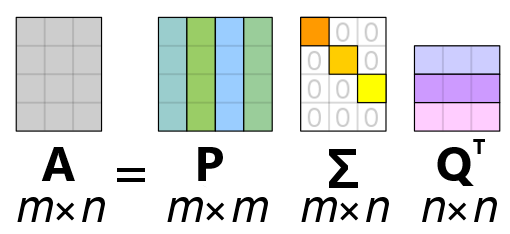
\includegraphics[scale=.5]{SVD.png}
        \\
        \caption{Adapted "\href{https://en.wikipedia.org/wiki/Singular_value_decomposition#/media/File:Singular_value_decomposition_visualisation.svg}{Visualization of SVD}" by \href{https://commons.wikimedia.org/wiki/User:Cmglee}{Cmglee} licensed under \href{https://creativecommons.org/licenses/by-sa/4.0/}{CC BY-SA 4.0} }
        \end{center}
    \normalsize
    \[ 
A = P \Sigma Q^T
\hspace{5mm}
\text{where}
\hspace{5mm}
\Sigma =
\left[
\begin{array}{ccc|c}
\sigma_1 & & & \\
& \ddots & & \boldsymbol{0} \\
& & \sigma_r & \\ \hline
& \boldsymbol{0} & & \boldsymbol{0}
\end{array} \right]_{m \times n}
\]
\subtopic{Construction}
$\sigma$ are known as the singular values of $A$.  We find them as the $\sqrt{\lambda}$ of either $AA^T$ or $A^TA$.  The columns and rows of $P$ and $Q$ are corresponding \emph{normalized} eigenvectors:
\vspace{-.4cm}
\begin{align*}
    A^TA \boldsymbol{q}_i = \sigma_i^2 \boldsymbol{q}_i & \qquad AA^T \boldsymbol{p}_i = \sigma_i^2 \boldsymbol{p}_i\\
    \boldsymbol{p}_i = \frac{1}{\sigma_i} A \boldsymbol{q}_i & \qquad \boldsymbol{q}_i = \frac{1}{\sigma_i} A^T \boldsymbol{p}_i
\end{align*}
Either $P$ or $Q$ may not have a full orthonormal basis defined based on the dimension and rank of $A$.  In these cases simply extend the basis to a full one by finding the remaining orthogonal subspace and applying GS algorithm.\\
\subtopic{Important Properties of SVD}
\vspace{-.5cm}
\small
\begin{align*}
    \mathrm{rank}(A) &= r\\
    \| A \| &= \sigma_1\\
    \| A^{-1} \| &= 1/\sigma_r\\
    \mathrm{cond}(A) &= \sigma_1 / \sigma_r\\
    \mathrm{null}(A) &= \mathrm{span} \{ \boldsymbol{q}_{r+1},\dots,\boldsymbol{q}_n \}\\
    \mathrm{range}(A) &= \mathrm{span} \{ \boldsymbol{p}_1,\dots,\boldsymbol{p}_r \}
\end{align*}
    
      
    
    
    
    \end{minipage}
};
%------------ SVD Decomposition ---------------------
\node[fancytitle, right=10pt] at (box.north west) {SVD Decomposition};
\end{tikzpicture}

%------------ PCA and Applications of SVD ---------------
\begin{tikzpicture}
\node [mybox] (box){%
    \begin{minipage}{0.3\textwidth}
    \subtopic{Principle Component Analysis}
    \small
    Create a data matrix $X$ composed of row vectors, the same shape as used for least squares fitting.  Normalize data so the columns have a mean value of 0.  Apply SVD decomposition to the data matrix, the principle weight vectors are the $q$ vectors.  We can project X onto its principle components to reduce the dimension of the data while keeping the most significant weight vectors of dimensioning.
    \newline
    \normalsize
    \subtopic{Pseudo Inverse}
    \vspace{-.2cm}
    \[A^+ = Q \Sigma^+ P^T\]
    \[
\Sigma^+ =
\renewcommand{\arraystretch}{1.25}
\left[ \begin{array}{ccc|c}
\sigma_1^{-1} & & & \\
& \ddots & & \boldsymbol{0} \\
& & \sigma_r^{-1} & \\ \hline
& \boldsymbol{0} & & \boldsymbol{0}
\end{array} \right]_{n \times m}
\renewcommand{\arraystretch}{1}
\]

\subtopic{SVD Expansion}
\[A = \sum_{i=1}^r \sigma_i \boldsymbol{p}_i \boldsymbol{q}_i^T = \sigma_1 \boldsymbol{p}_1 \boldsymbol{q}_1^T + \cdots + \sigma_r \boldsymbol{p}_r \boldsymbol{q}_r^T\]
    
    


    
    \end{minipage}
};
%------------ PCA and Applications of SVD ---------------------
\node[fancytitle, right=10pt] at (box.north west) {PCA and Applications of SVD};
\end{tikzpicture}

%------------ Complex Linear Algebra  ---------------
\begin{tikzpicture}
\node [mybox] (box){%
    \begin{minipage}{0.3\textwidth}
    \subtopic{Inner Product}
    \vspace{-.4cm}
    \begin{align*}
    <\bs{v},\bs{w}> = v_0\overline{w_0} & + v_1\overline{w_1} + \cdots + v_n\overline{w_n}\\
   <c\bs{v},\bs{w}> = c<\bs{v},\bs{w}> & \qquad <\bs{v},\bs{w}> = \overline{<\bs{w},\bs{v}>}\\
    <\bs{v},c\bs{w}> = \overline{c}<\bs{v},\bs{w}> & \qquad <\bs{v},\bs{v}> = ||\bs{v}||
\end{align*}

    \subtopic{Complex Analogs}
    Hermitian: $A=\overline{A}^T$\\
    Unitary: $A^{-1}=\overline{A}^T$\\
    If $A$ is hermitian then diagonal entries of $A$ are real
    \subtopic{Roots of Unity}
    The Nth complex roots of 1:\\
    \large
    $\omega = e^{\frac{2\pi i k}{N}}$ for $0<k<N, k\in \mathbb{C}^N$
    \normalsize
    
    
    \end{minipage}
};
%------------ Complex Linear Algebra ---------------------
\node[fancytitle, right=10pt] at (box.north west) {Complex Linear Algebra};
\end{tikzpicture}


%------------ Discrete Fourier Transform ---------------
\begin{tikzpicture}
\node [mybox] (box){%
    \begin{minipage}{0.3\textwidth}
    \subtopic{Fourier Basis}
    The fourier basis of $\mathbb{C}^N$ is an orthogonal basis defined as $\boldsymbol{f}_0 , \dots, \boldsymbol{f}_{N-1}$:
\[\renewcommand{\arraystretch}{1.5}
\boldsymbol{f}_k = \begin{bmatrix} 1 \\ \omega^k_N \\ \omega^{2k}_N \\ \vdots \\ \omega^{(N-1)k}_N \end{bmatrix}
\renewcommand{\arraystretch}{1} \]
\vspace{-.3cm}
\[\overline{\boldsymbol{f}}_k = \boldsymbol{f}_{N-k}\]
\subtopic{Fourier Transform}
\[\mathrm{DFT}(\boldsymbol{x}) = F_N \boldsymbol{x} \textrm{ and } F_N =\]
\small
\[
\renewcommand{\arraystretch}{1.5}
\begin{bmatrix} & & \overline{\boldsymbol{f}}^T_0 & & \\ & & \overline{\boldsymbol{f}}^T_1 & & \\ & & \vdots & & \\ & & \overline{\boldsymbol{f}}^T_{N-1} & & \end{bmatrix}
=
\renewcommand{\arraystretch}{1.25}
\begin{bmatrix}
1 & 1 & 1 & \cdots & 1 \\
1 & \overline{\omega}_N & \overline{\omega}_N^2 & \cdots & \overline{\omega}_N^{N-1} \\
1 & \overline{\omega}_N^2 & \overline{\omega}_N^4 & \cdots & \overline{\omega}_N^{2(N-1)} \\
1 & \vdots & \vdots & \ddots & \vdots \\
1 & \overline{\omega}_N^{N-1} & \overline{\omega}_N^{2(N-1)} & \cdots & \overline{\omega}_N^{(N-1)^2}
\end{bmatrix}
\renewcommand{\arraystretch}{1}
\]
\normalsize
Note that $\frac{1}{\sqrt{N}}F_N$ is unitary\\
\[
\boldsymbol{x}
= \frac{1}{N}
\begin{bmatrix} & & \\ \boldsymbol{f}_0 & \cdots & \boldsymbol{f}_{N-1} \\ & & \end{bmatrix}
\renewcommand{\arraystretch}{1.5}
\begin{bmatrix} & & \overline{\boldsymbol{f}}^T_0 & & \\ & & \overline{\boldsymbol{f}}^T_1 & & \\ & & \vdots & & \\ & & \overline{\boldsymbol{f}}^T_{N-1} & & \end{bmatrix}
\renewcommand{\arraystretch}{1}
\boldsymbol{x}
\]
Let $\boldsymbol{y} = \mathrm{DFT}(\boldsymbol{x})$ then:\\
\vspace{-.3cm}
\[\overline{\boldsymbol{y}[k]} = \boldsymbol{y}[N-k]\]
\subtopic{Inverse Transform}
\[
\mathrm{IDFT}(\boldsymbol{y}) = \frac{1}{N} \overline{F}^T_N \boldsymbol{y}\]


    
    \end{minipage}
};
%------------ Discrete Fourier Transform ---------------------
\node[fancytitle, right=10pt] at (box.north west) {Discrete Fourier Transform};
\end{tikzpicture}

\vspace{5cm}
%------------ DFT Analysis ---------------
\begin{tikzpicture}
\node [mybox] (box){%
    \begin{minipage}{0.3\textwidth}
    \subtopic{Sinusoids}
    For $N$ number of samples over a time period of 1, we have:
    \[
\boldsymbol{n} = \begin{bmatrix} 0 \\ 1 \\ 2 \\ \vdots \\ N-1 \end{bmatrix}
\hspace{10mm}
\boldsymbol{t} = (1/N) \boldsymbol{n} = \begin{bmatrix} 0 \\ 1/N \\ 2/N \\ \vdots \\ (N-1)/N \end{bmatrix}
\]
A discrete sinusoid signal is $\boldsymbol{x} = A \cos(2\pi k \boldsymbol{t} + \phi)$\\

The $k$th Fourier vector has the following sinusoidal properties:
\begin{align*}
\boldsymbol{f}_k & = \cos(2 \pi k \boldsymbol{t}) + i \sin(2 \pi k \boldsymbol{t}) \\
\frac{1}{2} \left( \boldsymbol{f}_k + \overline{\boldsymbol{f}}_k \right) &= \cos(2 \pi k \boldsymbol{t}) \\
\frac{1}{2i} \left( \boldsymbol{f}_k - \overline{\boldsymbol{f}}_k \right) &= \sin(2 \pi k \boldsymbol{t})
\end{align*}

For $\boldsymbol{x} = A \cos(2 \pi k \boldsymbol{t} + \phi)$:
\[
\mathrm{DFT}(\boldsymbol{x}) = \frac{AN}{2} e^{i \phi} \, \boldsymbol{e}_k + \frac{AN}{2} e^{-i \phi} \, \boldsymbol{e}_{N-k}
\]
\subtopic{Stemplots}


    
    \end{minipage}
};
%------------ DFT Analysis ---------------------
\node[fancytitle, right=10pt] at (box.north west) {DFT Analysis};
\end{tikzpicture}





\end{multicols*}

\end{document}


Contact GitHub API Training Shop Blog About
© 2016 GitHub, Inc. Terms Privacy Security Status Help